\def\year{2017}\relax
%File: formatting-instruction.tex
\documentclass[letterpaper]{article}
\usepackage{aaai17}
\usepackage{times}
\usepackage{helvet}
\usepackage{courier}
\usepackage{epsfig}
\usepackage{graphicx}
\usepackage{amsmath}
\usepackage{amssymb}
\usepackage{dsfont}
\usepackage{tablefootnote}
\usepackage{multirow}
\usepackage{subcaption}
\usepackage[ruled]{algorithm2e}

\frenchspacing
\setlength{\pdfpagewidth}{8.5in}
\setlength{\pdfpageheight}{11in}
% \pdfinfo{
% /Title (Semi-supervised Zero-Shot Learning by a Clustering-based Approach)
% /Author (Seyed Mohsen Shojaee and Mahdieh Soleymani Baghshah)}
% \pdfinfo{
% /Title (Insert Your Title Here)
% /Author (Put All Your Authors Here, Separated by Commas)}
\setcounter{secnumdepth}{0}
\newcommand{\norm}[1]{\left \lVert #1 \right \rVert_{F}^2}
 \newcommand{\etal}{\textit{et al.} }
\DeclareMathOperator*{\argmax}{arg\,max}
\DeclareMathOperator*{\argmin}{arg\,min}
\DeclareMathOperator*{\minimize}{min}
 \begin{document}
% The file aaai.sty is the style file for AAAI Press
% proceedings, working notes, and technical reports.
%
\title{Semi-supervised Zero-Shot Learning by a Clustering-based Approach}
 \author{Seyed Mohsen Shojaee {\normalfont and} Mahdieh Soleymani Baghshah\\
 Sharif University of Technology \\
 Tehran, Iran\\
 {\tt\small mshojaee@ce.sharif.edu, soleymani@sharif.edu}
 }

\maketitle
%\thispagestyle{empty}
%!!!!!!!!!!!!!!!!!!!!!!!!!!!!!!!!!!!!!!!!!!!!!!!!!! Content______________________________________________________________________________________________________

\begin{abstract}
In some of object recognition problems, labeled data may not be available for all categories.
 Zero-shot learning utilizes auxiliary information (also called signatures)
 describing each category in order to find a classifier that can recognize samples
from categories with no labeled instance. %RR It is usually only unseen classes
In this paper, we propose a novel semi-supervised zero-shot learning method that works on an embedding space corresponding to
abstract deep visual features. We seek a linear transformation on signatures to map them onto the visual features,
such that the mapped signatures of the seen classes are close to labeled samples of the corresponding
classes and unlabeled data are also close to the mapped signatures of one of the unseen classes.
 We use the idea that the rich deep visual features provide a representation
 space in which samples of each class are usually condensed in a cluster. The effectiveness of the proposed method is demonstrated through extensive
experiments on four public benchmarks improving the state-of-the-art prediction accuracy on three of them.
\end{abstract}


\section{Introduction}
Zero-shot learning \cite{bengio08,hinton09,lampert09,farhadi09} is an extension to the conventional supervised learning scenario
that does not need labeled instances for all categories in order to recognize them.
Instead, some sort of description that is called \textit{class signatures} is available for all the categories.
Signatures may be a set of human-annotated discriminative attributes or textual description of the categories.
The problem addressed by zero-shot learning rises naturally in practice wherever it is not feasible to acquire abundant labeled instances for
 all the categories (e.g., fine-grained classification problems).
To describe the task more precisely, in the training phase, labeled instances for some categories which are called seen classes are provided
while for other categories, called unseen ones, there is no labeled instance available.
In the test phase, unlabeled instances should be classified into seen or unseen categories.
 In this work, we focus on the most popular version of zero-shot recognition in which test instances belong only to unseen categories.
 %In this setting, zero-shot learning mitigates the problem of acquiring labeled instances, which can be hard for a novel, rare or fine-grained categories.
 \begin{figure}[!t]
 \begin{center}
 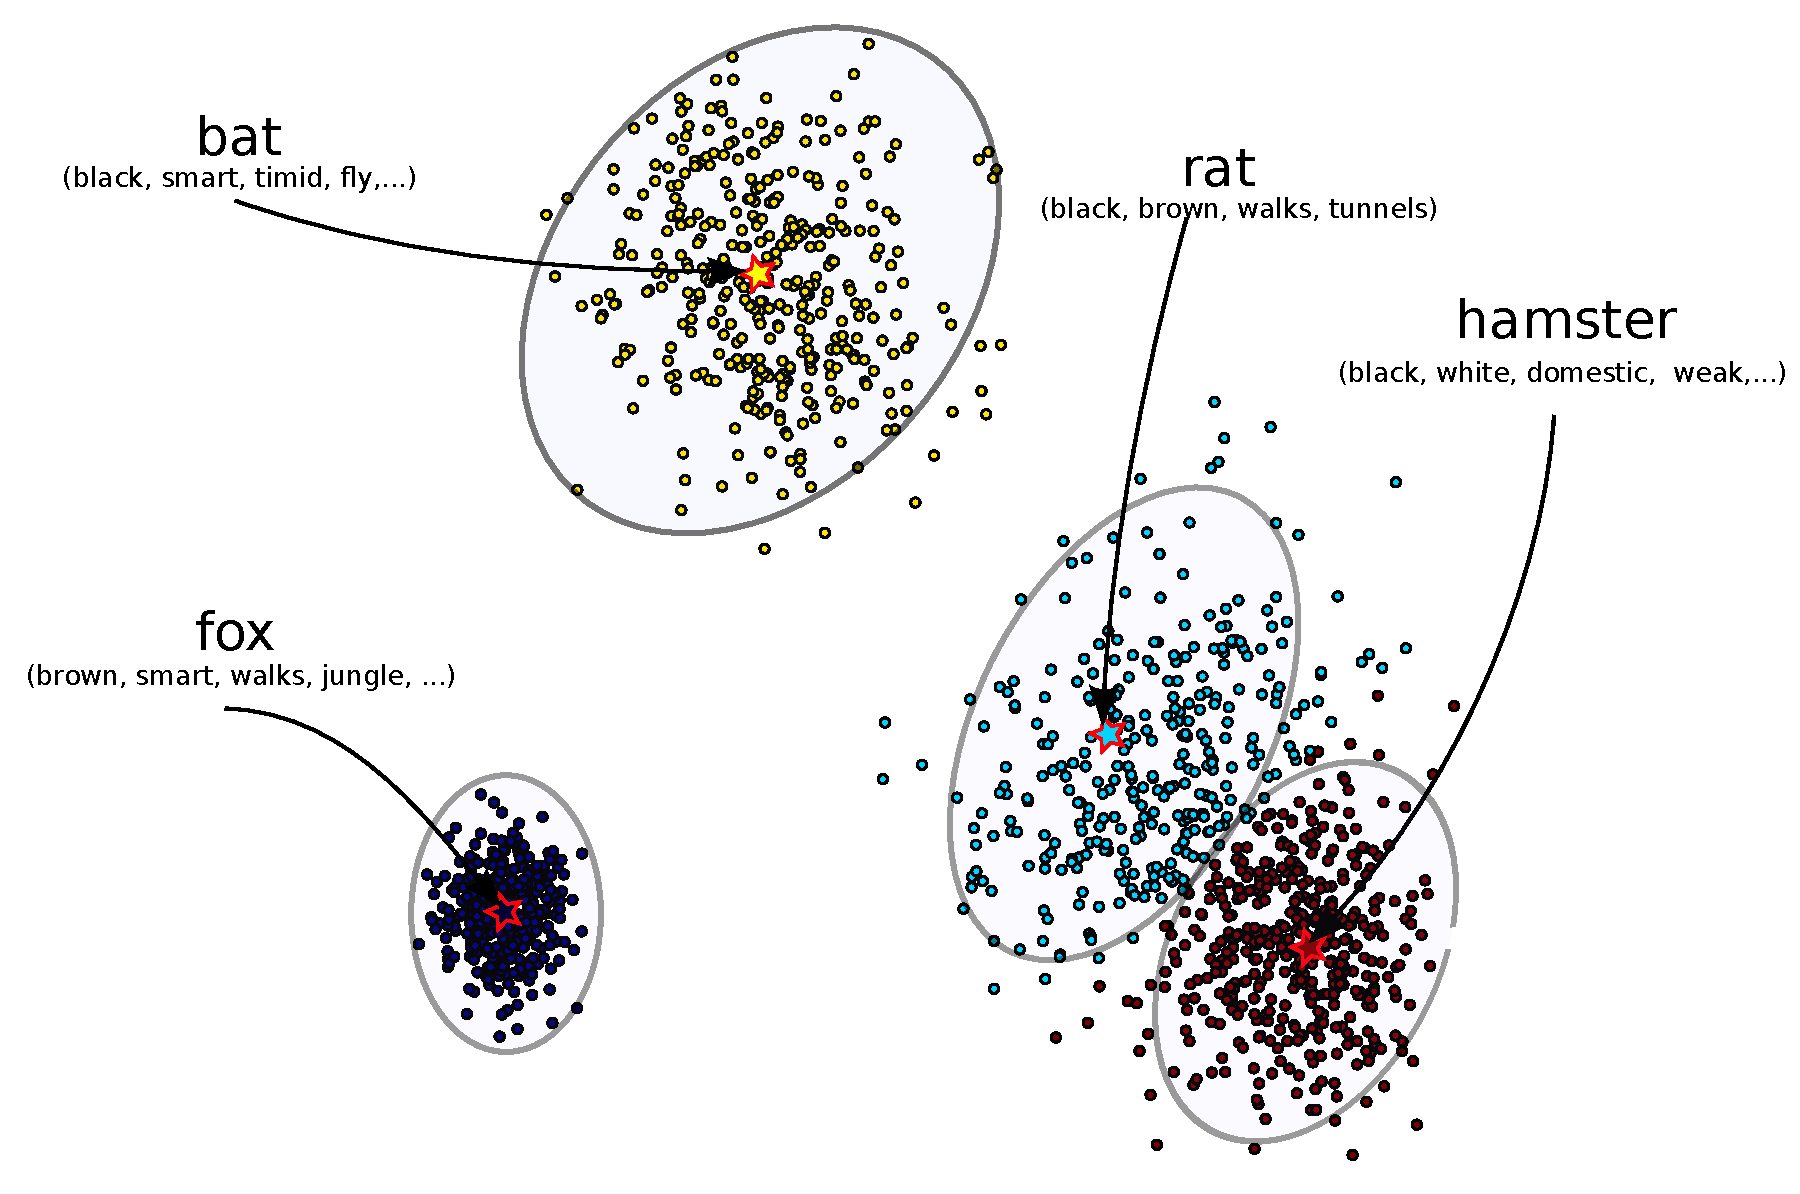
\includegraphics[width=0.98\columnwidth]{overview.pdf}
 \caption{In our model we map class signatures close to all instances of the class for seen classes and close to instances in a cluster for unseen ones.
 Three different clusters are shown here by circles with different colors and class signatures are mapped to center of clusters shown by stars of the same color}
 \label{fig:overview}
 \end{center}
 \vspace{-8mm}
 \end{figure}

Most existing methods for zero-shot learning focus on using labeled images to learn a compatibility function indicating how similar an image is
to each label embedding~\cite{Akata2015,emb15,sse}. Each instance will then be labeled with the category having the most compatible signature.
 On the other hand, recent advances in deep neural networks provide rich visual features with high discrimination capability~\cite{vgg}.
We will show in Section\ref{experiments} through experiments that the space of deep visual features is indeed a rich space
 in which instances of different categories usually form natural clusters.
Little attention has been paid to exploiting this property of visual features in the context of zero-shot learning.

 %In the previous works, most concentration has been on finding embeddings for visual features and little effort has been made to exploit unsupervised information in images domain.

In this paper, we propose Joint Embedding and Clustering (JEaC),
a semi-supervised zero-shot learning method in which both supervised information from labeled samples
and unsupervised information from unlabeled samples are utilized.
In this method the assignment of unlabeled samples to unseen classes is jointly learned
with a linear embedding from class signatures to the space deep image features (Figure~\ref{fig:overview} ).
The linear mapping is learned such that the mapped signature of each seen class tends to be representative
for samples of the corresponding class and simultaneously
assignments of unlabeled samples to unseen classes are leaned such that the mapped signature of each unseen class
 also tends to be the representative of the assigned samples to that class.
Using the unlabeled samples of the unseen classes, we can substantially mitigate
 \textit{the domain shift problem} introduced in \cite{eccv14} that impairs the zero-shot recognition performance.
%To show the capability of our proposed method that jointly learns the linear transformation on class signatures and label assignments to unlabeled data, we also propose simpler methods that do not use these ideas altogether. Indeed, we also propose two simpler methods that only optimizes one of these two objectives and also a method that considers both of these objectives but does not simultaneously optimizes them. Indeed, after finding the mapping, it uses a clustering algorithm to assign samples of unseen classes to those classes. A semi-supervised clustering algorithm is proposed for this purpose to leverage labels available for seen classes to obtain more accurate cluster assignments.
We also propose \textit{Independent Embedding and Clustering} (IEAC),
a simpler method in which label assignment and class embedding in image space are not learned joitly.
Instead, after finding the mapping using only samples from seen classes,  a clustering algorithm is used to assign labels to instances of unseen classes.
 %A semi-supervised clustering algorithm is proposed for this purpose to leverage labeled instances available for seen classes to obtain more accurate cluster assignments.

In Section~\ref{experiments}, we present experimental results on four popular zero-shot classification benchmarks
 and see that the proposed method outperforms the state-of-the-art methods on three out of these four datasets.

The rest of paper is organized as follow. In Section~\ref{related}, we briefly introduce existing methods for zero-shot learning.
In Section~\ref{proposed}, we present our semi-supervised zero-shot learning method. In Section \ref{experiments}, we report our experiments and finally in Section~\ref{conclusion}
we conclude.

%___________________________________________________________________________________________________________________________________________________________
%______________________________________Related Work_________________________________________________________
\section{Related Work} \label{related}
Most existing methods for zero-shot object recognition can be described as finding a compatibility function scoring how
similar an image and a description are.
We can consider three tasks for these methods:
  1) Find (or use the existing) embeddings for class labels in a semantic space.
  2) Map images into that semantic space.
  3) Classify images in the semantic space based on the compatibility of the mapped image and the embedded labels in this space (usually using a nearest neighbor classifier or label propagation).
Learning of these three steps may be done independently or jointly.

A notable body of work in zero-shot recognition belongs to attribute prediction from images \cite{lampert09,topicmodel,ajoint11,unified13,suzuki14}.
In these methods, the semantic label embeddings are considered to be externally provided attributes as auxiliary information. Thus, attributes as label embeddings are available and the task is just to map images to the semantic space, i.e., predicting attributes for the images.
Early methods, like \cite{lampert09}, assume independence between attributes and train binary attribute classifiers.
Probabilistic graphical models have been utilized to model and/or learn correlations among different attributes \cite{topicmodel,unified13} to improve the prediction of the attributes.
In \cite{jayaraman14}, a random forest approach has been employed that accounts for unreliability in attribute predictions for final class assignment.
In \cite{Akata2015pami}, a max-margin objective function similar to the structured SVM is defined for attribute-based image classification.
% When the label embeddings are fixed, it can be used for zero-shot recognition.

More recent works exploit bilinear models \cite{Yu2013,devise,convex,sse,emb15,semi15} that are also equivalent to embedding images and labels into a
common space and considering the inner product in the embedded space as the compatibility score.
Until now, several objective functions have been proposed for learning such bilinear models.
In \cite{emb15}, the sum of the squared error on the label prediction is used.
However, extra regularization terms that compensate undesirable characteristics of this cost function are also utilized.
This method can be seen as learning a mapping that transforms description of each class to a linear classifier for that class.
This idea has also been used in \cite{li15max,semi15} that introduce a max margin objective function for this purpose.
 These two methods also learn labels for test instances simultaneously and so they differ from almost all of other existing methods in this way. This provides the possibility of
leveraging unsupervised information available in test images, for instance as done in \cite{semi15}, by using a Laplacian regularization term that penalizes similar objects assigned to different classes.

Designing label embeddings in multi-class classification
% that can be considered as a general framework for multi-class classification
is another line of research that can also be used for zero-shot recognition.
 % For a label embedding to be helpful in classification tasks,
 % it should exhibit two properties \cite{Yu2013}: 1) category-separability and 2) learnability.
 In \cite{Yu2013}, an objective function is proposed to derive such label embeddings based on information about similarities among categories.
A relatively popular embedding for labels is to describe unseen categories as how similar they are to the seen ones.
One way to use this embedding is creating classifiers for unseen categories by linear combination of
classifiers for seen categories using similarity scores as mixing weights.
In \cite{convex}, the outputs from the softmax layer of a CNN trained on seen categories are used to score similarity between test instances and seen classes.
Using these outputs as weights, the introduced method in \cite{convex} represents images in the semantic space as a convex combination of seen class label embeddings.
Moreover, in \cite{sse}, a histogram showing seen class proportions is used for label embedding and then a max margin framework is defined to embed images in this space. The authors of \cite{convex} extend their work further in \cite{agnostic} and formulate a supervised dictionary learning method that jointly learns image and label embeddings.
 The idea of combining already available classifiers to create new ones for unseen categories is also used in \cite{Synthesized}
 but rather than using seen categories as basis, they define a set of (possibly smaller) \textit{phantom} classes and learn base classifiers on them.

 Although most of the studies on zero-shot recognition consider attributes as auxiliary information, some of the existing methods utilize textual
  information for classes as auxiliary information.
  This text be obtained from online encyclopedias or be just the name of classes.
   Some existing methods first extract features from auxiliary text information and then turn them into vectors that can be treated analogous to attribute vectors.
 \cite{devise} introduces a bilinear model to find the compatibility score of deep visual features and Word2vec \cite{word2vec} representation of class names. \cite{ba2015} proposes nonlinear mappings modeled by neural networks on the image and the text inputs to find their compatibility.
  \cite{mohamed13} presents an objective function to predict classifier parameters from textual descriptions. In \cite{Akata2015}, different label embeddings such as attribute vectors, GloVe \cite{pennington2014glove}, word2vec \cite{word2vec}, a variant of word2vec with weak supervision, and also a combination of these different embeddings have been considered as the label embedding for zero-shot recognition. In \cite{Xian2016}, this work is extended further to model nonlinear compatibility
   functions that can be expressed as a mixture of bilinear models.
   % Intuitively, different linear models will use different aspects of images to measure the compatibility and the proper aspect is selected automatically for every test image.s
  In \cite{Qiao2016}, a modification of \cite{emb15} is presented as for use with textual auxiliary information by decomposing the bilinear mapping.

In \cite{Fu2016}, a set of vocabulary much larger than just seen and unseen class names is used and mapping from images to word embeddings is learned
by  maximizing the margin with respect to all words in the vocabulary; this framework can be used in zero-shot and also supervised and open set learning problems.
In  \cite{Akata2016}, authors propose to use multiple auxiliary information and also  part annotation in image domain to compensate for weaker supervision in textual data.
%The nature of zero-shot learning problem in which usually only one document exists for each category has hindered using more sophisticated models for text embedding.
Convolutional and recurrent neural networks  have also been used for text embedding in \cite{Akata2016rnn}.

The most related methods to our method are the introduced ones in \cite{li15max,Kodirov2015,semi15}
 that are indeed semi-supervised zero-shot learning methods. Here, we briefly specify the differences between these methods and ours. First, we use abstract visual features obtained by deep learning as the semantic space as opposed to these methods. \cite{li15max,semi15}
learn a max margin classifier on the image space classifying both seen and unseen instances while we use a ridge regression to map signatures to the semantic visual space resulting in a much simpler optimization problem to solve. Since samples of different classes are usually condensed in distinct regions of the deep visual representation space, our proposed optimization problem is based on clustering of data in this space and we try to map the class signatures on the centroid of the corresponding samples. We also explicitly account for domain shift problem in our objective function and thus achieving better results compared to these methods.

There are major differences between our work and ~\cite{Kodirov2015} using a dictionary learning scheme
in which coding coefficients are considered to be label embeddings in a semantic space
and a sparse coding objective is used to map images into this representation space.
Most importantly, in our method labels of unseen instances are jointly learned
with the mapping of the signatures to the semantic space in our objective function while in \cite{Kodirov2015}
the label prediction is accomplished using the nearest neighbor or the label propagation on embeddings of images.
Also, we do not need to learn embedding of test instances in the semantic space as opposed to \cite{Kodirov2015},
alternatively we learn just the representation of class signatures in the visual domain.

\section{Proposed Approach} \label{proposed}
In this section, we introduce two zero-shot learning method that use the deep visual features as the semantic space and learns
a mapping from class signatures to this semantic space and also predict labels for instances belonging to unseen classes.
 First, we propose Independent Embedding and Clustering (IEaC), a simple and efficient semi-supervised zero-shot learning method in Section~\ref{clustering}.
Then, we further extend our method to jointly learn the embedding of signatures and class assignments of unlabeled samples.
We call this method Joint Embedding and Clustering (JEaC). We formulate JEaC as an optimization problem and
 introduce an iterative method to solve this it in Section~\ref{optimization}.
 We use IEaC to find a starting point for this optimization procedure (i.e., as an initial labellings for instances of unseen classes).
\subsection{Notation}
Let $X, \mathbf{x}$, and $x$ denote matrices, column vectors, and scalars respectively. $\norm{X}$ shows the squared Frobenius norm of a matrix and
$X_{(i)}$ denotes its $i$th column. $\mathbf{1}_k$ denotes a column vector whose $k-th$ element is one and is zero everywhere else.
Suppose there are $n_s$ seen categories and $n_u$ unseen categories. For each category y,
auxiliary information $a_y \in \mathbb{R}^r$ is available. We assume that labels $\{1, \ldots, n_s \}$ correspond to seen categories.

Let $X_s \in \mathbb{R}^{d \times N_s}$ and $X_u \in \mathbb{R}^{d \times N_u}$
denote matrices whose columns are seen and unseen images respectively where $d$ is the dimension of image features.
$S_s = [a_1, \ldots, a_{n_s}]$ presents the matrix of signatures for seen classes. $S_u$ is also defined similarly for unseen classes.
$Z_s = [ \mathbf{z_1}, \ldots, \mathbf{z_{N_s}} ]$
contains labels of training data in one-hot encoding format.

\subsection{Clustering Method} \label{clustering}
Our first method can be roughly summarized in three steps:
\begin{enumerate}
  \item Using data from seen classes, we learn a linear mapping from attribute vectors to the semantic space.
  \item We find a data clustering using our proposed semi-supervised clustering algorithm.
  \item For instances of each cluster, we find the label whose mapped signature in the semantic visual space is the nearest one to the center of that cluster and assign that label to all of these instances.
\end{enumerate}

We use a simple ridge regression to map class signatures to visual features. We intend to find a mapping from class signatures
 to the deep visual representation space such that each mapped (seen) class signature is close to the samples of that class in this space in average.
The linear mapping is found using the following optimization problem:
\begin{equation} \label{eq:mapping}
  D = \argmin_D \norm{X_s - D Y_s} + \gamma \norm{D},
\end{equation}
where columns of $ Y_s \in \mathbb{R}^{r \times n_s} $ are the class signatures of the samples lied in the columns of $X_s$.
This optimization problem is known to have the following closed form solution:
\begin{equation} \label{eq:dic}
  D = X_s Y_s^T (Y_s Y_s^T + \gamma I)^{-1}.
\end{equation}
The parameter $\gamma$ is determined through cross validation as we will describe precisely in Section~\ref{experiments}.

Here, we intend to find labels for instances belonging to unseen classes. To this end, we want to find a clustering of instances
 in the space of deep visual features and assign a label to each cluster according to the distance between the center of that cluster
 and the mapped signature of the unseen classes
(i.e., consider the label whose mapped signature is the closest one to the cluster center as the assigned label to the instances of this cluster).
To find a better clustering of instances belonging to unseen classes,
 we can also incorporate labeled instances of seen classes too.
  The clustering problem over unseen instances, we encountered here, is different from the conventional semi-supervised learning problem \cite{chapel06}.
In fact, all labeled data are from seen classes and there is no labeled sample for unseen classes that is due to the special characteristic of zero-shot learning problem. Therefore, here, we propose a semi-supervised learning method which
can be seen as an extension to k-means suitable for this problem.
 We try to find a clustering such that labeled instances tend to be assigned to the corresponding classes and all instances tend to be close to the center of the clusters to which they are assigned:
\begin{equation} \label{eq:simple}
\minimize_{R, \mathbf{\mu_1, \ldots, \mu_k }}  \sum_{n,k} r_{nk} \lVert \mathbf{x_n - \mu_k} \rVert_2^2 +
 \beta \sum_{n=1}^{N_s} \mathds{1}(\mathbf{r_n \neq z_n}),
\end{equation}
where $\mathbf{\mu_i'}$s are cluster centers and $R = [\mathbf{r_1, \ldots, r_{N_s + N_u }} ]$ is cluster assignments in one-hot encoding format.
The objective function is similar to that of the k-means clustering algorithm but for each labeled instance there is a penalty of $\beta$ if its assigned cluster number that is different from its label. Thus, this objective function encourages
the first $n_s$ clusters be corresponding to the seen classes.
%This is intuitively plausible, on one hand all data is being used in the clustering and on the other ????????

Parameters $\beta$ and $k$ can be determined via the cross validation. However, in our experiments, we found out
the model is not very sensitive to these so we fix $\beta=1$
when data is normalized such that $\lVert x_i \rVert_1 = 1$. We set $k =  (n_s + 2n_u)$, this
will allow for two clusters per class for unseen categories. This, to some extent, copes with diversity in instances of a class.


Finally, to assign labels to test instances, we use the mapping $D$ from Eq.\eqref{eq:dic} to
map class signatures to visual features, creating a set of \textit{class representatives}
 in the visual feature space. We then assign to all instances of a cluster the class label whose representative is
  the nearest to center of that cluster.
%We argue that the this method of assigning labels to clusters rather than individual instances can mitigate the domain shift problem in zero-shot learning.

% We argue that this learning scheme can mitigate domain shift problem  between seen and unseen categories and thus achieve higher classification accuracy.

%This is specifically favorable in our setting where we want to use this mapping to classify cluster centers that also approximate \textit{average} of class instances.

%Because all members of each cluster is assumed to share the same label. To overcome this bottleneck, in the next section we present a joint frame work to learn cluster assignments jointly with the mapping.
A key distinction between the clustering-based method presented here and other existing methods lies in the nature of the compatibility function.
 The compatibility function in other works is a similarity measure between each instance and class description that is found independently for different instances.
 Here, the compatibility function relies strongly on the distribution of instances in the semantic space and the compatibility of a label for an instance is found according to the similarity of the cluster center to which this instance is assigned and the mapped signature of that label. Therefore, by considering the distribution of data points (via clustering)
  in designing the compatibility function we can reach a more reliable measure.
  This compatibility function can be plugged in every other method in this way that after final predictions are made by the method,
a clustering algorithm is ran on data and then we assign an identical label to all cluster
members by majority voting on those predictions. We found through experiment that this extra step will improve performance of
many existing methods.

Although the above method outperforms the state-of-the-art methods on most zero-shot recognition benchmarks, it uses only the instances of the seen classes to find the linear transformation from class signatures to the visual feature space and thus the proposed method may suffer from the domain shift problem introduced in \cite{eccv14}.
To overcome the domain shift problem more substantially, we propose an optimization problem for finding the linear transform from class signatures to the visual feature space that uses instances of both seen and unseen classes.

\subsection{Joint Embedding and Clustering}
\label{joint}
%In the method we proposed earlier, once the the points are assigned to a cluster, they all will inevitably share an identical label. This can limit the performance of the method. One example arises for cluster \textit{outliers} that are distant from center of their cluster but lie nearby a landmark. This instances most probably belong to the class of nearby landmark but will be labeled same as their cluster center. To overcome this issue we propose a framework to learn the mapping jointly with cluster assignments  (which will be reported as label predictions at the end).  While allowing more flexibility, this framework abates the domain shift problem in the same way as the previous method.
 In this section, we propose an optimization problem for learning a linear transformation from class signatures to the visual features space such that
 the mapped signatures are good representatives of the corresponding instances.
 We intend to learn a transformation such that for the seen classes, the sum of the squared distances of instances from the
 mapped signature of the corresponding class is minimized. Moreover,
for instances of unseen classes, we can find class assignments such that the sum of the squared distances of unseen instances from the mapped signature
of classes to which they are assigned is also minimized.
 The objective function of JEaC is formulated as follows:
 \begin{align} \label{eq:main}
   \minimize_{R,D} \norm{X_s - D Y_s}  &+ \lambda \norm{X_u - D S_u R^T } + \gamma \norm{D} \\
   \text{s. t.} \quad & R \in \{0,1\}^{N_u \times n_u}. \nonumber
 \end{align}
The first term in the above optimization problem is identical to Eq.\eqref{eq:mapping} and the second one incorporates unlabeled data for learning the mapping $D$. By enforcing
 the signatures to be mapped close to test instances, this term confronts the domain shift problem. In fact, we seek a class assignment for instances of unseen classes such that we can learn a linear transformation on class signature to use the mapped signature of both seen and unseen classes as good representatives for the corresponding instances.
 The second term can be essentially considered as a clustering objective with two advantages. First, the number of clusters is no longer a
 parameter and it is determined by the number of unseen classes. Second, the cluster centers are set to be the mapped signatures of test classes.

\subsection{Optimization} \label{optimization}
\begin{algorithm}[t]
  {\small
  \SetKwData{Left}{left}\SetKwData{This}{this}\SetKwData{Up}{up}
\SetKwFunction{Union}{Union}\SetKwFunction{FindCompress}{FindCompress}
\SetKwInOut{Input}{input}\SetKwInOut{Output}{output}
  \Input{ $X_s, Y_s, Z_s, X_u, S_u$}
  \Output{$Z_u$ (label predictions for $X_u$)}
$k \in \{ 1,2, \ldots, n_s + n_u \}$\\
  $n \in \{ 1,2, \ldots, N_s + N_u \}$ \\
  \BlankLine
  Initialize $\boldsymbol{\mu_k}$ by Eq. \eqref{eq:updata_mu}, $k=1,\ldots,n_s$\;
  Initialize $\boldsymbol{\mu_k}$ by kmeans++, $k=n_s+1,\ldots,n_s+n_u$\;
 \Repeat{convergence to local minimum}{
    $ c_n \leftarrow  {\argmin_i \lVert x_n - \mu_i \rVert_2};$  //cluster assignments\\
    $\mathbf{\mu_k} \leftarrow \sum_{n} \mathbf{x_n} \mathds{1}(c_n = k) / \sum_n (\mathds{1}(c_n = k) $ \;
 }
 $  D \leftarrow X_s Y_s^T (Y_s Y_s^T + \gamma I)^{-1}$\;
 // array $l$ maps cluster numbers to labels
 $l[k] \leftarrow \argmin_j \lVert \mathbf{\mu_k} - (DS_u)_{(j)} \rVert_2$\;
  $\mathbf{(Z_u)_{(n)}} \leftarrow \mathbf{1}_{l[c_n]}$\;
 }
 \caption{Training Procedure of IEaC }
 \label{alg:leca}
\end{algorithm}
\vspace{3mm}

\textbf{Training Algorithm for IEaC: } %Linear Embedding with Cluster Assignment
Optimization of  the objective function in Eq.~\eqref{eq:simple} is done by alternating between
$\mathbf{\mu_i'}$s and R. $\mathbf{\mu_i'}$s are updated using:
\begin{equation} \label{eq:updata_mu}
  \mu_i = \frac{\sum_{n=1}^{N_s + N_u}  \mathds{1}(r_{ni}=1)\mathbf{x_n}}{\sum_{n=1}^{N_s+N_u}\mathds{1}(r_{ni}=1)},
\end{equation}
$R$ is updated by assigning each instance  to the cluster that minimizes the corresponding term in Eq.\eqref{eq:simple}.
To initialize $\mathbf{\mu_i'}$s, for clusters corresponding to seen classes the centers are set as mean of instances from that class. Centers of other
clusters are initialized using k-means++ \cite{kmeanspp} on unlabeled instances.
The overall training algorithm IEaC is presented in algorithm \ref{alg:leca}

\textbf{Training algorithm for JEaC: }
The Eq.~\eqref{eq:main} is not convex and considering that $R$ is a partitioning of instances, the global optimization requires an
exhaustive search over all possible labeling of test data with $n_u$ labels. Therefore, we use a simple coordinate descent
method (like k-means). We alternate between optimizing $R$ and $D$ while fixing the other.
Having fixed the labeling $R$, the problem becomes a simple multi-task ridge regression which has the following closed-form solution:
\begin{equation} \label{eq:d_update}
  D = (X_s Y_s^T + \beta X_u R S_u^T) (Y_s Y_s^T + \beta S_u R^T R S_u^T  + \gamma I)^{-1}.
\end{equation}
By fixing $D$, the optimal $R$ can be achieved via assigning each instance to the closest class representative:
\begin{equation} \label{eq:r_update}
  r_{ij} = \mathds{1}[j = \argmin_{k} \lVert X_{u(i)} - D S_{u(k)} \rVert_2 ].
\end{equation}
Whenever a row of $R$ contains no 1's, i.e.  an empty cluster is encountered we assign 2\% of instances randomly to that cluster.
We continue alternating between updates of $D$ and $R$ till R remains constants, i.e., no label changes. In our experiments, this always happens
in less that 20 iterations.

To evade poor local minima, we use a good starting point that initilizing $R$ with prediction made by IEaC.
\begin{algorithm}[t]
   \label{alg:jeac}
  {\small
  \SetKwData{Left}{left}\SetKwData{This}{this}\SetKwData{Up}{up}
\SetKwFunction{Union}{Union}\SetKwFunction{FindCompress}{FindCompress}
\SetKwInOut{Input}{input}\SetKwInOut{Output}{output}
  \Input{ $X_s, Y_s, Z_s, X_u, S_u$}
  \Output{$Z_u$ (label predictions for $X_u$)}
  \BlankLine
  Initialize $R$ by output of Algorithm \ref{alg:leca} \;
 \Repeat{no element of $R$ changes}{
    update $D$ by Eq. \eqref{eq:d_update} \;
    updata $R$ by Eq. \eqref{eq:r_update} \;
 }
  output $Z_u \leftarrow R$
 }
 \caption{Training Procedure for JEaC}
\end{algorithm}

\section{Experiments} \label{experiments}

\begin{table*}[ht]
\begin{minipage}{\textwidth}
\centering
\caption{Accuracy score (\%) of cluster assignments converted to labels
using majority voting on ground truth labels on four zero-shot recognition benchmarks.
Results are our method are average $\pm$ std of three runs.
} \vspace{2mm} \label{tab:cluster}
\begin{tabular}{|l|c|c|c|c|}
\hline
Clustering Method & Animals with Attributes & CUB-2011 & aPascal-aYahoo & SUN Attribute \\
\hline
k-means                             &  65.80                 & 35.61           & 65.37                & 17.49    \\
\hline
Proposed Clustering                     & \textbf{70.74$\pm$0.32}  & \textbf{42.63$\pm$0.07} & \textbf{69.93$\pm$ 3.4} & \textbf{ 45.50$\pm$1.32} \\
\hline
\end{tabular}
\vspace{2mm}
\end{minipage}
\end{table*}

\begin{table*}[ht]
\begin{minipage}{\textwidth}
\centering
\caption{Classification accuracy in \% on four public datasets: Animals with Attributes, CUB-2011, aPascal-aYahoo and SUN
in form of average $\pm$ std.
} \vspace{2mm} \label{tab:results}
\begin{tabular}{|l|l|c|c|c|c|}
\hline
Feature & Method & Animals with Attributes & CUB-2011 & aPascal-aYahoo & SUN \\
\hline
{Shallow}
&  \cite{li15max}                 &  38.2$\pm$2.3   &                 &                         & 18.9$\pm$2.5 \\
& \cite{semi15}                    &  40.05$\pm$2.25 &                 &   24.71 $\pm$3.19       &     \\
& \cite{jayaraman14}  &43.01 $\pm$ 0.07 &                 & 26.02 $\pm$ 0.05        & 56.18 $\pm$ 0.27 \\
\hline
{GoogleNet}
& \cite{Akata2015}              & 66.7            & 50.1            &                         & \\
& \cite{Synthesized}       & 72.9            & 54.5            &                         & 62.7 \\
& \cite{Xian2016}                & 71.9            & 45.5            &                         & \\
\hline
{VGG-19}
&  \cite{Kodirov2015}
                                            & 73.2            &  39.5           & 26.5                    &  \\
& \cite{Akata2015}              & 61.9            &  50.1           &                         & \\
&  \cite{sse}            &  76.33$\pm$0.53 & 30.41 $\pm$0.20 &   46.23 $\pm$ 0.53      & 82.50 $\pm$ 1.32    \\
& \cite{agnostic}       &  80.46$\pm$0.53 & 42.11 $\pm$0.55 &   \textbf{50.35 $\pm$ 2.97}      & 83.83 $\pm$ 0.29    \\

& IEaC (k-means)                             & 86.34$\pm$0.13               & 52.48$\pm$0.60              & 48.03$\pm$1.56              & 75.75$\pm$1.06 \\
& IEaC (Proposed Clustering)                             & 86.38$\pm$0.56               & 53.10$\pm$0.43              & 48.00$\pm$0.69              & 80.66$pm$0.76 \\
& JEaC (init D)                     & 83.03                        & 57.55                       & 42.62          & 72.50\\
& JEaC (init R)                     & \textbf{\em 88.64$\pm$0.04}  & \textbf{\em 58.80$\pm$0.64} & 49.77$\pm$2.02 & \textbf{\em 86.16$\pm$0.57} \\
\hline
\end{tabular}
\end{minipage}\vspace{-3mm}
\end{table*}
In this section, we conduct experiments on the popular benchmarks to obtain results of the proposed method on these benchmarks and compare them with those of the other methods.

\textbf{Datasets.}
We evaluate our proposed methods on four popular public benchmarks for zero-shot classification.
(1) Animal with Attributes (AwA) \cite{lampert09}. There are images of 50 mammal species in this data set
Each class is described by a single $85-$dimensional attribute vector. We use the continuous attributes rather than
the binary version as it has proved to be more discriminative in previous works like \cite{Akata2015}. The train/test split provided by the dataset is used accordingly.
(2) aPascal/aYahoo \cite{farhadi09}. The 20 categories from Pascal VOC 2008 \cite{pascal} are considered as seen classes and
categories from aYahoo are considered to be unseen. As this dataset provides instance level attribute vectors,
for class signatures we use the average of the provided instance attributes.
(3) SUN Attribute \cite{sun}. The dataset consists of 717 categories and all images are annotated with 102 attributes, we just
use the average attributes among all instances of each categories for our experiments. We use the same train/test spilt
as in \cite{jayaraman14} where 10 classes have been considered unseen.
(4) Caltech UCSD Birds-2011 (CUB) \cite{cub}. This a dataset for fine-grained classification task. There are 200 species of
birds where each image has been annotated with 312 binary attributes. Again, we average over instances to get continuous class signatures.
We use the same train/test split as in \cite{akata13} (and many other following works) to make comparison possible.

As our method relies on meaningful structure in visual features domain, we use features from a deep CNN known that are
 more discriminative than \textit{shallow} features like SIFT or HOG. We report results using
  $4096-$dimensional features from the first fully connected layer of 19 layer VGG network \cite{vgg}
pre-trained on image-net, provided publicly by \cite{sse}.
%We also report results using 2) $1024-$dimentional features from GoogleLeNet \cite{googlenet} provided publicly by \cite{Akata2015}.
\begin{figure*}[t]
  \centering
  \begin{subfigure}[b]{0.27\linewidth}
    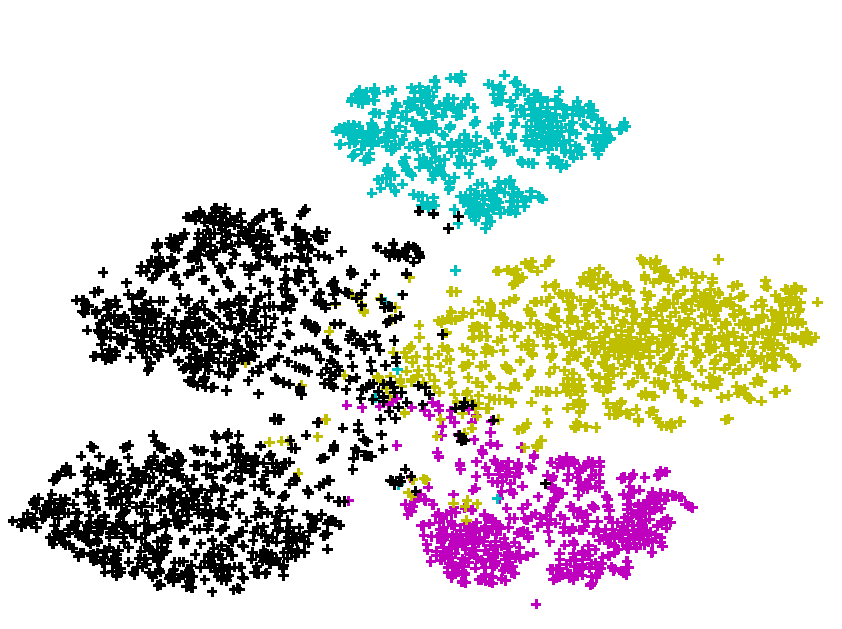
\includegraphics[width=\linewidth]{figure_1}
    \caption{}
    \label{fig:null}
  \end{subfigure}
%
  \begin{subfigure}[b]{0.27\linewidth}
    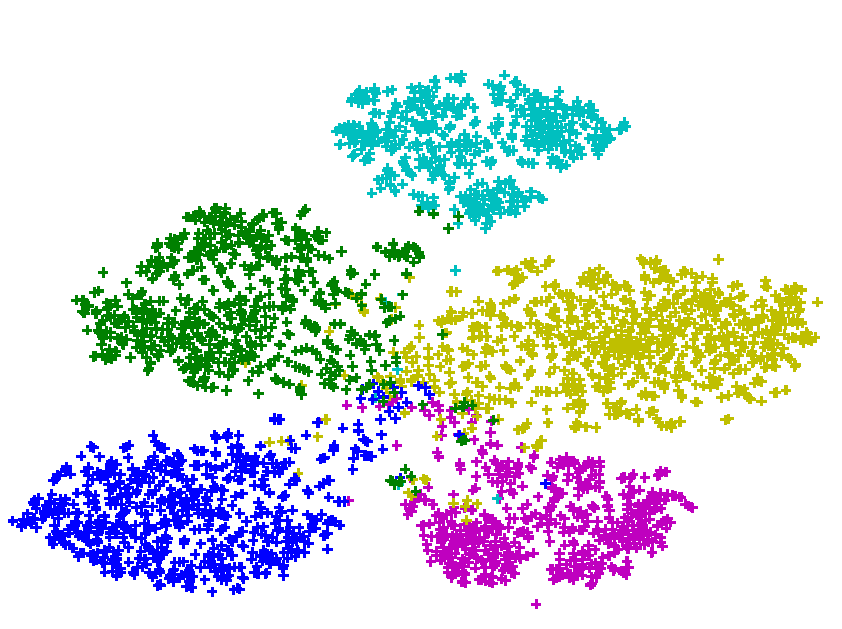
\includegraphics[width=\linewidth]{figure_1_true}
    \caption{}
% \caption{Points colored according to their ground truth labels}
    \label{fig:truth}
  \end{subfigure}
%
  \begin{subfigure}[b]{0.27\linewidth}
    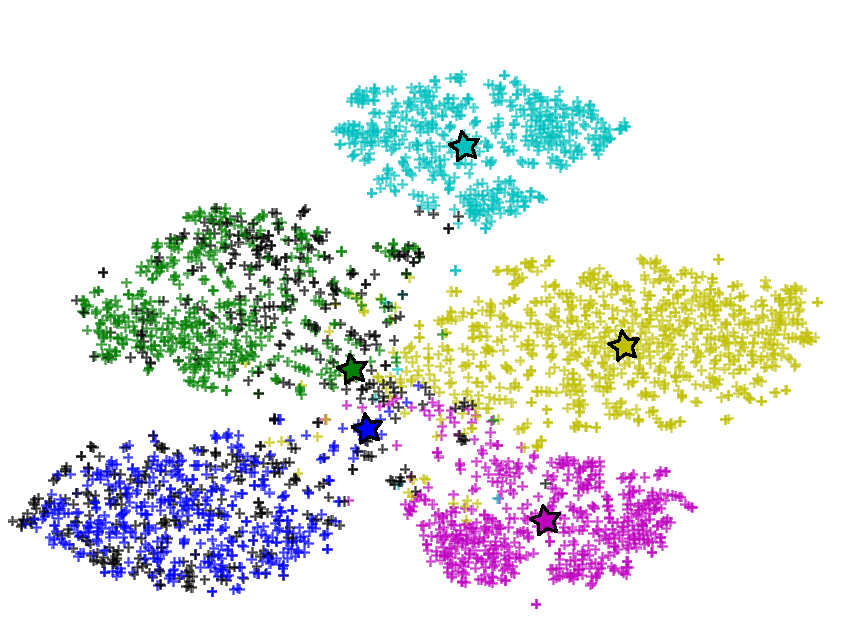
\includegraphics[width=\linewidth]{figure_2}
    % \caption{Signatures mapped to image spacing using Eq. \eqref{eq:dic} and denoted by stars. Then classification done using nearest neighbor}
    \caption{}
\label{fig:knn}
  \end{subfigure}
%
  \begin{subfigure}[b]{0.27\linewidth}
    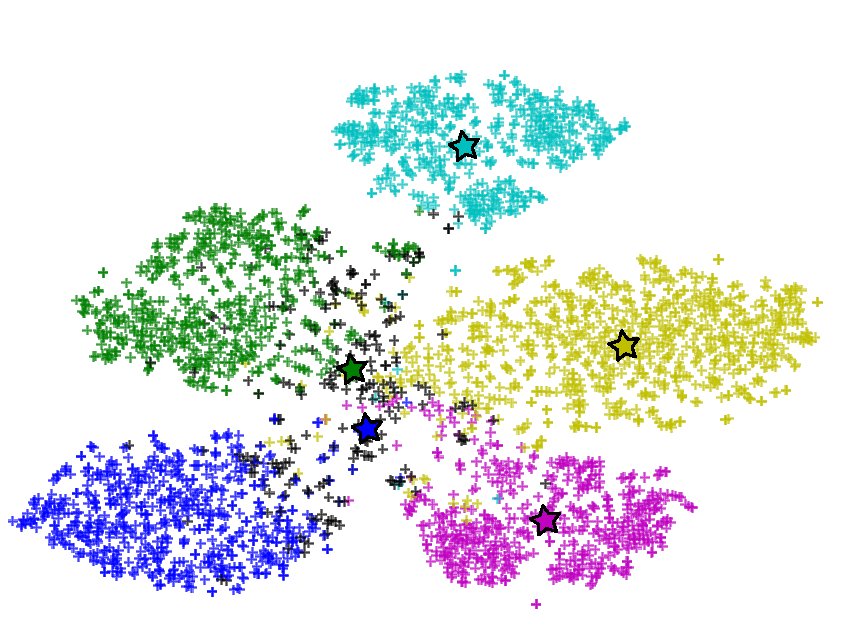
\includegraphics[width=\linewidth]{figure_3_kmeans}
    % \caption{Stars as previous. Classification done by our compatibility function on cluster assignments from k-means}
    \caption{}
\label{fig:kmeans}
  \end{subfigure}
%
  \begin{subfigure}[b]{0.27\linewidth}
    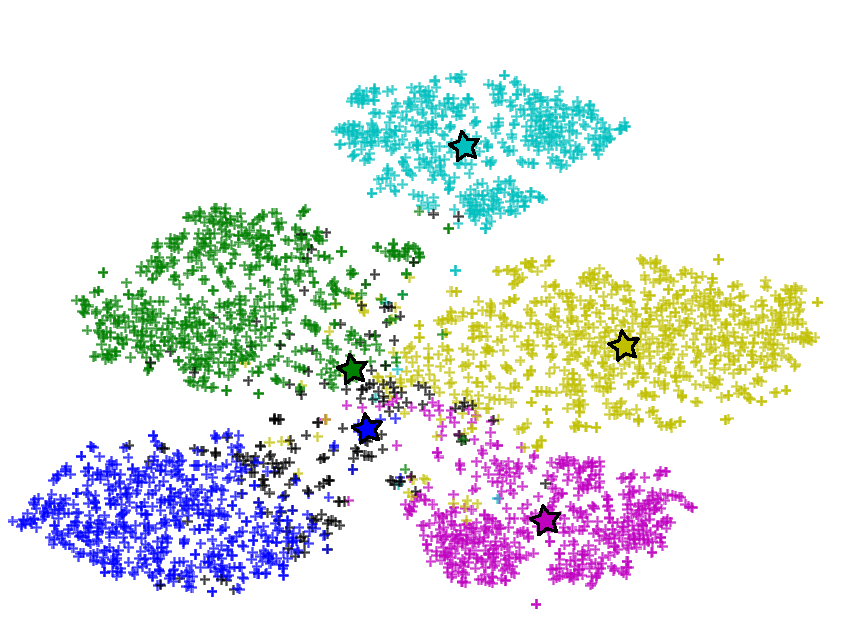
\includegraphics[width=\linewidth]{figure_3}
    \caption{}
    \label{fig:clustering}
% \caption{Stars as previous. Classification by our compatibility function using our supervised clustering}
  \end{subfigure}
%
  \begin{subfigure}[b]{0.27\linewidth}
    \label{fig:joint}
    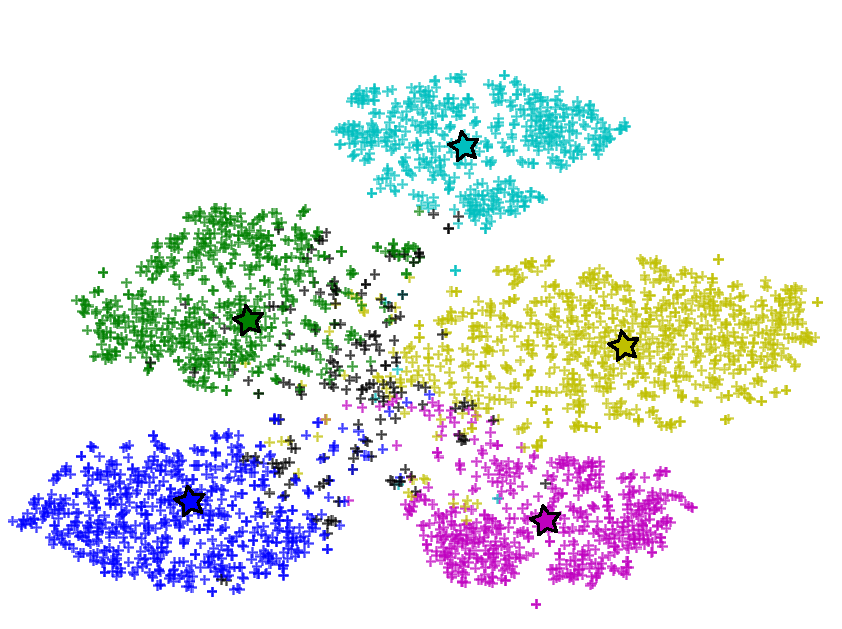
\includegraphics[width=\linewidth]{figure_4}
    \caption{}
% \caption{Class signatures mapped to image space (stars) and cluster assignment by JEaC}
  \end{subfigure}
  \caption{t-SNE embedding of five classes from AwA, three seen: antelope (magenta), grizzly bear (yellow), killer whale (cyan) and two
  unseen: chimpanzee (blue), giant panda (green). Images shown by plus signs and embedding of class signatures in images space by stars.
  in figures b-f black points denote assignment to a class other five classes shown here.
  \textbf{b)} Points colored according to their ground truth labels
  \textbf{c)} Signatures mapped to image spacing using Eq. \eqref{eq:dic}. Then classification done using nearest neighbor
  \textbf{d)} Classification done by our compatibility function on cluster assignments from k-means
  \textbf{e)} Classification by our compatibility function using our supervised clustering
  \textbf{f)} Class signatures mapping and cluster assignment by JEaC
  }
  \label{fig:tsne}
\end{figure*}

\textbf{Testing Cluster Assumption:}
First, to give evidence for our key assumption of our method that instances from each class usually form a cluster in visual feature domains
and to demonstrate effectiveness of our proposed clustering algorithm we design an
experiment in which instances from unseen categories are clustered using our proposed clustering algorithm and also the k-means algorithm. Then,
each cluster is assigned with a class label based on majority voting on ground truth labels. The number of clusters
 is set to the number of classes as a natural choice.
 \footnote{However we found out through experiment that increasing the number of clusters improves the accuracy.}
For the k-means algorithm, we use the implementation available in Scikit-learn library \cite{scikit-learn} and run it with 20 different initializations
and report results of that one with the best score.
Accuracy of this labeling scheme that is based on clustering is reported in Table~\ref{tab:cluster}.
These results shows the effectiveness of our proposed clustering method and that the cluster structure assumption in the visual semantic space is usually right.

\textbf{Cross Validation:}
To adjust parameters $\gamma$ and $\beta$ in Eq.~\ref{eq:d_update} and parameter $\gamma$ in Eq. \ref{eq:dic}, we split training data into train and validation sets.
We choose a number of categories randomly from training data as validation categories. For each data set, the size of the
validation set has the same ratio to the train set as the size of the test categories to the total of the train and the validation one.
In our experiments, we used $10-$fold cross validation, i.e., average results from ten different validation splits are used to decide on
optimal parameters.
Once optimal $\gamma$ and $\beta$ are determined through the grid search by testing on validation set, the model
is then trained on all seen categories.

We summarize our experimental results in Table~\ref{tab:results}.
\textit{IEaC (Proposed Clustering)} corresponds to the method presented in Section~\ref{clustering}.
\textit{IEaC ( K-means)} is another version of our simple  method in which our semi-supervised clustering is substituted by k-means clustering.
\textit{JEaC(init D)} and \textit{JEaC(init R)} correspond to optimizing Eq.~\eqref{eq:main}
with respectively initializing $D$ using Eq.~\eqref{eq:dic} and initializing $R$ by IEaC.
For our methods, average and standard deviation of different runs are reported. As it can be seen, the initialization done
by IEaC has critical effect on the performance. This can be justified by noting the information from structure of
unlabeled data is leveraged when initializing $R$ while such information is absent in initializing $D$.

 For other methods, we use the results reported in their original publication. Note that some experimental settings of these works may differ from those of ours. We did not re-implement any of the other methods and if the original paper does not report results on a data set we leave the corresponding cell as blank.
Our method performs the best on three out of the four datasets (outperforms the others on all except to the aPascal-aYahoo dataset). This can be explained by the nature of the dataset in which class signatures obtained by averaging instance attributes are very similar. We suppose trying to learn
more discriminative signatures from data can potentially improve the result. We investigate this in our future work.

The effectiveness of different components of our methods in further illustrated in Figure~\ref{fig:tsne}. As it can be seen in
Figure~\ref{fig:knn} merely using mapping from Eq. \eqref{eq:dic} results in poor signature embeddings where domain shift problem is
visible. However using the compatibility function based on cluster assignments, although the there is no change in mappings,
label assignments are improved, our clustering  (Figure~\ref{fig:clustering} ) performing  better than k-means (Figure~\ref{fig:kmeans}). Finally using
mapping from JEaC, the domain shift problem is substantially alleviated and far better signature embeddings are achieved.



% We implemented our method using scikit-learn library \cite{scikit-learn} in Python.
% \footnote{Code is available at online :-?}
%  and used an Intel Core i5 CPU at 3.2 GHz to run the experiments.

\section{Conclusion} \label{conclusion}
In this paper, we proposed semi-supervised methods for zero-shot object recognition.
We used the space of deep visual features as a semantic visual space and learned a linear transformation to map class signatures to this
space such that the mapped signatures provide good representative of the corresponding instances.
We utilized this property that the rich deep visual features provide a representation space in which samples of each class
are usually condensed in a cluster. In the proposed method that jointly learns the mapping of class signatures and the class assignments of unlabeled data,
we used also unlabeled instances of unseen classes when learning the mapping to alleviate the domain shift problem.
Experimental results showed that the proposed method generally outperformed the other recent methods.
%\section*{Acknowledgement}
{\small
\bibliographystyle{aaai}
\bibliography{semi_zsl.bib}
}

\end{document}
